\documentclass[11pt]{article}
    %	options include 12pt or 11pt or 10pt
    %	classes include article, report, book, letter, thesis
    
    \title{HW2}
    \author{Shane Drafahl}
    \date{8 September ,2017}
    \usepackage{graphicx}
    \usepackage{epstopdf}
    \usepackage{graphics}

    \begin{document}
    \maketitle

    1. Define a DFA, simplified to the best of your abilities, 
    to recognize the language L = $ \{\ a^{i}b^{i} : $ (i + j) mod 3 = 0 $ \}\  $
    $ \newline \newline $
    
    \begin{figure}[!htb]
        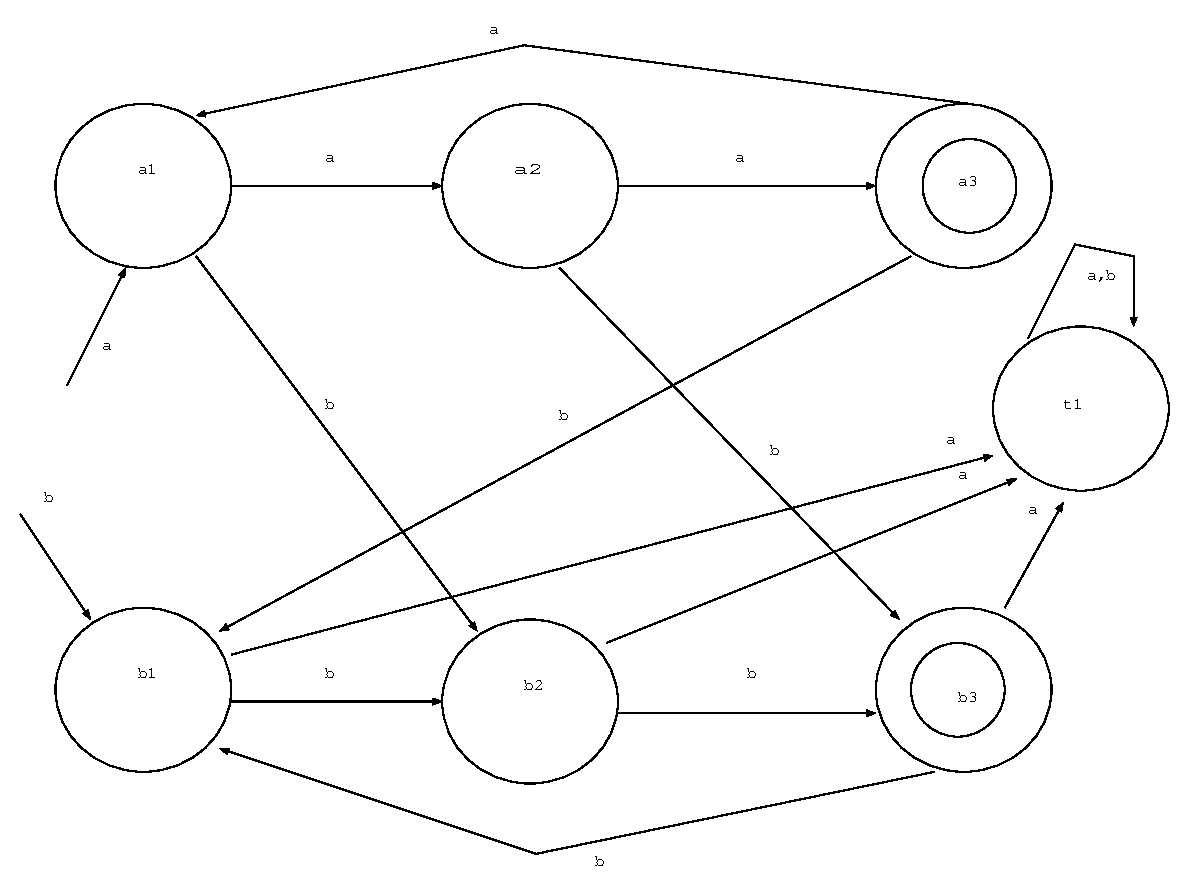
\includegraphics[scale=.7]{./hw2_1.eps}
    \end{figure}

    $ \newline \newline $

    2. Describe in a short English sentence the language accepted by the following DFA, and give a
    regular expression for it (hint: the “names” of the states reflect their meaning). Then, define
    a 5-state NFA that accepts the same language.

    $ \newline \newline $

    This DFA takes in characters from a alphabet of $ \Sigma $ = $ \{\ 1,0 \}\ $.
    From left to right they are concatentated into binary numbers. The string must end with 
    4 binary numbers that are inclusive values between 0-7 after converting the last 4 binary numbers
    into decminal values. 
    $ \newline \newline $
    Regular expression: $ (0 + 1)^{*}0(0 + 1)(0 + 1)(0 + 1) $
    $ \newline \newline $
    \begin{figure}[!htb]
        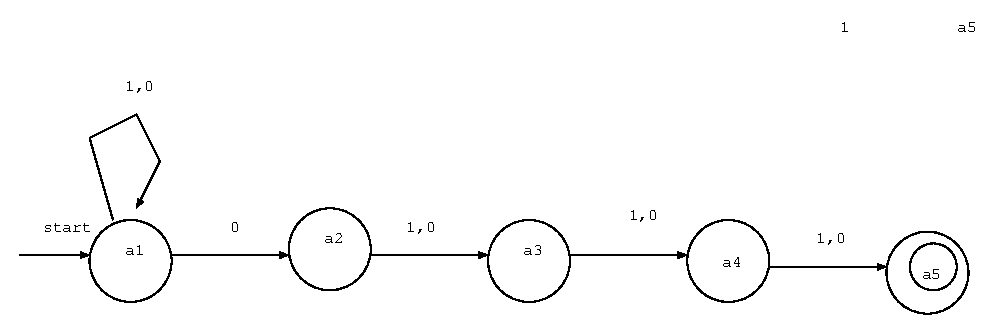
\includegraphics[scale=.7]{./hw2_2.eps}
    \end{figure}
    $ \newline \newline $
    3. Define a DFA equivalent to the following NFA.
    $ \newline \newline $
    \begin{figure}[!htb]
        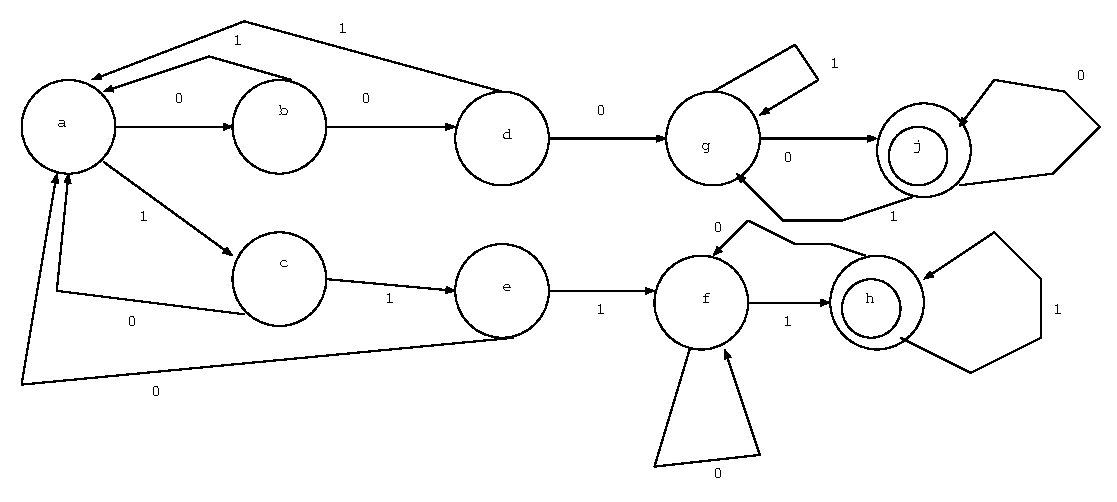
\includegraphics[scale=.7]{./hw2_3.eps}
    \end{figure}



    \end{document}